\documentclass{beamer}

\usepackage[utf8]{inputenc}
\usepackage[brazilian]{babel}
\usepackage[ruled,vlined]{algorithm2e}

\title{Hashes Camaleão de Pré-Imagem Pós-Quânticas baseadas em
Reticulados}
\author{Thiago Leucz Astrizi}
\institute{UFSC}
\date{2020}
\setbeamertemplate{footline}[frame number]

\begin{document}

\frame{\titlepage}

\begin{frame}
    \frametitle{Definições}
    \begin{block}{Função Hash}
    É um algoritmo eficiente $H$ junto com duas famílias de espaços: $M=\{M_{\lambda, \Lambda}\}_{\lambda, \Lambda}$ e $Y=\{Y_{\lambda, \Lambda}\}_{\lambda, \Lambda}$ onde $\lambda > 0$ é um inteiro chamado de parâmetro de segurança e 
    $\Lambda = P(\lambda)$ é uma string de bits que codifica os parâmetros de sistema obtidos pelo algoritmo de parametrização $P$. Cada par $(\lambda, \Lambda)$ onde $\Lambda = P(\lambda)$ identifica um único conjunto de $M$ e $Y$. O tamanho de $\Lambda$ é limitado por um polinômio sobre $\lambda$.
    \begin{itemize}
        \item $M$ e $Y$ devem ser eficientemente reconhecíveis.
        \item $H$ é um algoritmo eficiente, determinístico tal que $H(\lambda, \Lambda, msg) = dgt$ com $msg\in M_{\lambda, \Lambda}$ e $dgt \in Y_{\lambda,\Lambda}$.
    \end{itemize}
    \end{block}
    A probabilidade de um adversário $\mathcal{A}$ encontrar uma colisão em $H$ é dada em função de $\lambda$ e representada por CRadv$[\mathcal{A}, H](\lambda)$. Se esta é uma função negligível para todo $\mathcal{A}$ ($\forall c>0$, $\lim_{\lambda\rightarrow\infty}\textrm{CRadv}[\mathcal{A}, H](\lambda)\cdot\lambda^c = 0$), então $H$ é resistente à colisão.
\end{frame}

\begin{frame}
    \frametitle{Definições}
    \begin{block}{Função de Trapdoor}
    Esquema formado por tupla de algoritmos $T=(KeyGen_T, F, F^{-1})$
    sobre  $(X, Y)$ com $X=\{X_{\lambda,\Lambda}\}_{\lambda, \Lambda}$ e $Y=\{Y_{\lambda, \Lambda}\}$:
    \begin{itemize}
        \item $X$ é eficientemente reconhecível e amostrável. 
        \item $Y$ é eficientemente reconhecível. 
        \item $KeyGen_T$: É algoritmo probabilístico eficiente invocado como  $(\mathcal{PK}, \mathcal{SK})\leftarrow^{\$}KeyGen_T(\lambda, \Lambda)$.
        \item $F$: Algoritmo eficiente e determinístico que recebe $\lambda$, $\Lambda$, $\mathcal{PK}$ e $x \in X_{\lambda,\Lambda}$. Retorna $y \in Y_{\lambda,\Lambda}$.
        \item $F^{-1}$: Algoritmo eficiente probabilístico, recebe $\lambda$, $\Lambda$, $\mathcal{SK}$ e $y \in Y_{\lambda,\Lambda}$. Retorna $x \in X_{\lambda,\Lambda}$ tal que $F(\lambda, \Lambda, \mathcal{PK}, x)=y$.
    \end{itemize}
    O esquema é de mão única se a probabilidade de todo adversário $\mathcal{A}$ que recebe $\lambda$, $\Lambda$, $\mathcal{PK}$ e $y \in Y_{\lambda,\Lambda}$ retornar um $x$ tal que $F(\lambda,\Lambda,\mathcal{PK}, x) = y$ é uma função negligível (OWadv$[\mathcal{A},T](\lambda)$). 
    \end{block}
\end{frame}

\begin{frame}
\frametitle{Definições}

\begin{block}{Hash Camaleão de Pré-Imagem}
    Esquema formado por tupla de algoritmos $CH=(KeyGen, Hash, PreImage)$ sobre $(M, R, D)$ com $M=\{M_{\lambda,\Lambda}\}_{\lambda, \Lambda}$, $R=\{R_{\lambda,\Lambda}\}_{\lambda, \Lambda}$ e $D=\{D_{\lambda,\Lambda}\}_{\lambda, \Lambda}$:
    \begin{itemize}
    \item $R$ deve ser eficientemente reconhecível e amostrável.
    \item $M$ deve ser eficientemente reconhecível.
        \item $KeyGen$: Probabilístico. Retorna $(\mathcal{PK}, \mathcal{SK})\leftarrow^{\$}KeyGen(\lambda,\Lambda)$.
        \item $Hash$: Determinístico, recebe $\lambda$, $\Lambda$, $\mathcal{PK}$, $msg\in M_{\lambda,\Lambda}$ e $rnd\in R_{\lambda,\Lambda}$ e retorna $dgt \in D_{\lambda,\Lambda}$
        \item $PreImage$: Probabilístico, recebe $\mathcal{SK}$, $msg \in M_{\lambda,\Lambda}$ e $dgt \in D_{\lambda,\Lambda}$. Retorna $rnd \in R_{\lambda,\Lambda}$ tal que $Hash(\mathcal{PK}, msg, rnd)=dgt$.
    \end{itemize}
    Para todo adversário eficiente $\mathcal{A}$ que recebe $\lambda$, $\Lambda$ e $\mathcal{PK}$, a probabilidade de encontrar $(msg, rnd)$ e $(msg', rnd')$ tal que eles sejam uma colisão em $Hash(\lambda, \Lambda, \mathcal{PK}, \cdot, \cdot)$ é negligível (e denotada por CCRadv$[\mathcal{A}, CH]$).
    \end{block}
\end{frame}

\begin{frame}
\frametitle{Construção de David Cash para Hash Camaleão}

\begin{block}{Definição dos Algoritmos}
Dada a função hash $H: M \rightarrow Y$, a função de trapdoor $T=(KeyGen_T, F, F^{-1})$ sobre $(X, Y)$ e existindo a definição de um grupo abeliano aditivo em $Y_{\lambda,\Lambda}$, definamos uma hash camaleão de pré-imagem $CH=(KeyGen, Hash, PreImage)$ sobre $(M, X, Y)$:

\begin{itemize}
    \item O parâmetro de segurança $\lambda$ de $CH$ será o mesmo a ser usado em $H$ e no esquema $T$.
    \item O parâmetro de sistema da hash camaleão $\Lambda$ deve ser formado pela concatenação dos parâmetros de sistema da função hash e do esquema de função com trapdoor.
    \item Omitindo os parâmetros $\lambda$ e $\Lambda$ das funções, definimos os algoritmos de $CH$ como:
    \begin{itemize}
        \item $KeyGen() = KeyGen_T()$
        \item $Hash(\mathcal{PK}, msg, rnd) = H(msg) - F(\mathcal{PK}, rnd)$
        \item $PreImage(\mathcal{SK}, msg, dgt) = F^{-1}(\mathcal{SK}, H(msg) - dgt)$
    \end{itemize}
\end{itemize}

\end{block}

\end{frame}

\begin{frame}{Construção de David Cash para Hash Camaleão}
   \textbf{Prova:}  Mostraremos que se  $rnd \in X_{\lambda,\Lambda}$ for igual a $PreImage(\mathcal{SK}, msg, dgt)$, então $Hash(\mathcal{PK}, msg, rnd) = dgt$:
   
   \begin{equation}
 \begin{split}
 Hash(\mathcal{PK}, msg, rnd) &= Hash(\mathcal{PK}, msg, F^{-1}(\mathcal{SK}, H(msg) - dgt))\\
 &= H(msg) - F(\mathcal{PK}, F^{-1}(\mathcal{SK}, H(msg) - dgt))\\
&= H(msg) - H(msg) + dgt\\
&= dgt\\
 \end{split}
 \end{equation} \qed

Obs: Mesmo que $H$ seja uma função hash resistente à colisão e $I=(KeyGen_I, F, F^{-1})$ seja um esquema de mão única, não necessariamente a hash camaleão obtida desta forma é resistente à colisão.

\end{frame}

\begin{frame}{Função Hash de Ajtai}

\begin{block}{Definição}
Dada uma matriz $A$ de inteiros módulo $q$ tal que $A \in
\mathbb{Z}_q^{n\times m}$, definimos a função hash de Ajtai como a função que mapeia vetores $\overrightarrow{msg} \in \{0,1\}^{m}$ para digests $t \in \mathbb{Z}_q^n$ da seguinte forma:

$$
H_A(\overrightarrow{msg}) = A\cdot \overrightarrow{msg} \mod q
$$
\end{block}

Definimos para esta função que o parâmetro de segurança $\lambda$ determina o número de linhas da matriz $A$. As dimensões da matriz $A$, o valor de $q$ e todos os valores dentro de $A$ deverão ser codificados no parâmetro de sistema $\Lambda$.

Para quais dimensões e valores de $q$ essa função seria resistente à colisão e além disso seria uma função de compressão?

%Para o caso específico $H_A(\overrightarrow{m}) = 0$, o conjunto de estradas que satisfaz isso está contida em um reticulado. Para $H_A(\overrightarrow{m}) = \overrightarrow{c}$, as entradas que satisfazem isso estão contidas em um reticulado ideal, ou um reticulado que foi transladado.


\end{frame}

\begin{frame}{Função Hash de Ajtai}

\begin{block}{Exemplo}
Para $n=2$, $m=7$ e $q=8$:

$\begin{bmatrix}5 & 2 & 1 & 1 & 1 & 4 & 2\\5&0&0&6&2&1&7\end{bmatrix}\times\begin{bmatrix}1\\1\\0\\0\\1\\0\\0\end{bmatrix}=\begin{bmatrix}0\\7\end{bmatrix}$
\end{block}

Notar que $|M_{\lambda,\Lambda}|=2^m$ e $|D_{\lambda,\Lambda}|=q^n$.

Para termos uma função de compressão, $2^m>q^n \implies m > n\lg q$.

O artigo ``\href{https://web.eecs.umich.edu/~cpeikert/pubs/swifftx.pdf}{SWIFFTX: A Proposal for the SHA-3 Standard}'' usa $n=64$, $q=257$ e $m=2048$ em sua construção.

\end{frame}

\begin{frame}{Reticulados}

\begin{block}{Definição}
 Um \textbf{reticulado} é um conjunto de pontos $n$-dimensionais com uma estrutura periódica. Dados $n$ vetores linearmente independentes
 $\overrightarrow{b_1},\ldots\overrightarrow{b_n} \in \mathbb{R}^n$
 o reticulado gerado por eles é o conjunto de vetores:
 
 $$
 \mathcal{L}(\overrightarrow{b_1},\ldots\overrightarrow{b_n})=\left\{\sum_{i=1}^nx_i\overrightarrow{b_i}
 : x_i \in \mathbb{Z}\right\}
 $$
 
 Os vetores $\overrightarrow{b_1},\ldots\overrightarrow{b_n}$ são a
 \textbf{base} do reticulado.
 \end{block}

 Um \textbf{reticulado ideal} é o resultado após somar todos os vetores de um reticulado a uma constante $\overrightarrow{c}$.
 
 Notar que o conjunto de vetores $\overrightarrow{msg}$ que são solução para $A\cdot\overrightarrow{msg} \mod q=0$ estão contidos em um reticulado. Já os vetores que são solução para $A\cdot\overrightarrow{msg} \mod q = \overrightarrow{c}$ para $\overrightarrow{c}$ constante, estão contidos em reticulado ideal.
\end{frame}

\begin{frame}{Short Integer Solution Problem (SIS$_{n, m, q, \beta}$)}
    
Dada $A \in \mathbb{Z}_q^{n \times m}$ com elementos que consistem em
$m$ vetores aleatórios uniformes como colunas, encontrar um vetor não-nulo 
$\overrightarrow{x} \in \mathbb{Z}^n$ tal que:

\begin{itemize}
    \item $||\overrightarrow{x}||\leq \beta < q$
    \item $A\overrightarrow{x}=\overrightarrow{0} \in \mathbb{Z}_q^n$
\end{itemize}

Para garantir a existência de soluções não-triviais, é necessário:

\begin{itemize}
    \item $\beta \geq \sqrt{n\log q}$
    \item $m \geq n \log q$
\end{itemize}

De acordo com nossa hipótese, a probabilidade de encontrar soluções para este problema é dada por uma função negligível sobre $n$.
\end{frame}

\begin{frame}{Short Integer Solution Problem (SIS$_{n, m, q, \beta}$)}
    O problema pode ser visto como encontrar vetor não-nulo em um reticulado m-dimensional que estejam dentro de uma esfera de raio $\beta$ centrada na origem. O valor $\beta$ deve ser grande o bastante para que existam soluções e pequeno o bastante para que elas não sejam fáceis de ser encontradas.
    
    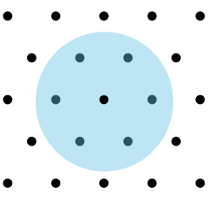
\includegraphics[height=2cm]{imagens/sis.png}
    
    Pela hipótese SIS, para todo $n$, $m$ e $q$ satisfazendo os requisitos, todo algoritmo que recebe $A\in\mathbb{Z}_q^{n\times m}$ aleatória e uniforme, só é capaz de encontrar $\overrightarrow{x}$ tal que $A\cdot \overrightarrow{x}=0$ com probabilidade negligível.
\end{frame}

\begin{frame}{Resistência à Colisão na Hash de Ajtai}
    \textbf{Teorema: }Se encontrar solução para o SIS só pode ser feito com probabilidade negligível, então a Hash de Ajtai ($H_A$) com $A$ é resistente à colisão, desde que sua matriz $A$ tenha parâmetros que na nossa hipótese torna o SIS difícil e $\beta \geq \sqrt{m}$.
    
    \textbf{Prova: }Para todo adversário $\mathcal{A}$ que tenta encontrar colisões em $H_A$, podemos gerar o algoritmo abaixo:
    
    \begin{algorithm}[H]
    \SetAlgoLined
    \KwIn{$n, m, q \in \mathbb{Z}, A\in\mathbb{Z}_q^{n \times n}$}
    \KwResult{Vetor pequeno $\overrightarrow{x}$ tal que $A\cdot\overrightarrow{x} \mod q = \overrightarrow{0}$}
    $\lambda \leftarrow n$\;
    $\Lambda \leftarrow$Encode$(n, m, q, A)$\;
    $(\overrightarrow{x_1},\overrightarrow{x_2})\leftarrow^{\$}\mathcal{A}(\lambda,\Lambda)$\;
    \textbf{return} $\overrightarrow{x_1}-\overrightarrow{x_2}$\;
    \caption{Solucionando o SIS}
\end{algorithm}
\end{frame}

\begin{frame}{Resistência à Colisão na Hash de Ajtai}

\textbf{Prova (cont.):} O algoritmo anterior retorna uma solução correta se, e somente se, $A \cdot (\overrightarrow{x_1}-\overrightarrow{x_2}) \mod q = \overrightarrow{0}$ e $(\overrightarrow{x_1}-\overrightarrow{x_2})< \beta$.

Para a primeira parte, se o adversário $\mathcal{A}$ realmente conseguiu encontrar uma colisão, então:

$$A\cdot\overrightarrow{x_1} \mod q= A\cdot\overrightarrow{x_2} \mod q$$

$$
A\cdot\overrightarrow{x_1} - A\cdot\overrightarrow{x_2} \mod q = \overrightarrow{0}
$$

$$
A\cdot(\overrightarrow{x_1} -\overrightarrow{x_2}) \mod q = \overrightarrow{0}
$$

Para a segunda parte, basta lembrar que se $\mathcal{A}$ encontrou uma solução, então $\overrightarrow{x_1}, \overrightarrow{x_2}\in\{0,1\}^m$. Portanto a diferença entre eles terá norma euclideana de no máximo $\sqrt{m}\leq\beta$. 
\end{frame}

\begin{frame}{Resistência à Colisão na Hash de Ajtai}
    \textbf{Prova (cont.): }Portanto, para todo adversário eficiente $\mathcal{A}$ que encontra colisões na Hash de Ajtai, podemos construir um algoritmo $\mathcal{B}$ também eficiente que resolve o problema SIS usando os mesmos parâmetros de matriz. E:
    
    $$
    Pr[\mathcal{B}\ \textrm{gera\ resposta\ correta}] \geq \textrm{CRadv}[\mathcal{A}, H_A](\lambda)
    $$
    
    Então se existe um adversário eficiente que encontra colisões com probabilidade não-negligível, existirá também um algoritmo que resolve o SIS com probabilidade não-negligível, o que por hipótese assumimos não ser possível.

    Portanto, a função hash de Ajtai é resistente à colisão.\qed

\end{frame}

\begin{frame}{Função com Trapdoor de Micciancio}
\begin{block}{Descrição}
Vamos descrever a Função com Trapdoor de Micciancio $T=(KeyGen_T, F, F^{-1})$ sobre $(X, \mathbb{Z}_q^n)$ onde $X$ é o conjunto de vetores pertencentes à $\mathbb{Z}_q^m$ com norma euclideana menor que $\beta$.

\begin{itemize}
    \item O parâmetro de segurança $\lambda$ será o número de linhas $n$ da matriz que iremos usar.
    \item Como parâmetro de sistema $\Lambda$ codifique os valores de $n$, $m$, $q$ e $\beta$ que serão usados.
    \item A chave pública $\mathcal{PK}$ será uma matriz $A\in\mathbb{Z}_q^{n \times m}$.
    \item  $F(\lambda,\Lambda,\mathcal{PK}, \overrightarrow{x})=A\cdot\overrightarrow{x} \mod q$.
    

    %\item Temos que ser capazes de inverter $F$. Então a matriz $A$ não pode ser uniforme e aleatória. Vamos assumir que existe um $G$ fácil de ser invertido.
    
    %\item Mas não podemos escolher $G=A$, pois inverter a função $F$ só pode ser feito para quem conhece o trapdoor.
    \end{itemize}
    
    O diferencial é que aqui devemos ser capazes de inverter a função $F(\lambda,\Lambda,\mathcal{PK}, \cdot)$.
    
    \end{block}
\end{frame}

\begin{frame}{Função com Trapdoor de Micciancio}
\begin{block}{Esolhendo um $A\in\mathbb{Z}_q^{n \times m}$}
\begin{itemize}
    \item $A$ não pode ser aleatoria e uniforme.

    \item Assumimos que exista $G\in\mathbb{Z}_q^{n \times w}$ específico para o qual para todo $\overrightarrow{y}\in\mathbb{Z}_q^n$ podemos achar $\overrightarrow{x}$ tal que $G\cdot\overrightarrow{x}=\overrightarrow{y}$.

    \item Não podemos usar $A=G$, pois nesse caso a função não seria de mão única como queremos.

    \item Mas isso torna-se possível com ajuda de um trapdoor $R \in\mathbb{Z}_q^{(m-w)\times w}$. Com ele podemos gerar um $A\in\mathbb{Z}_q^{n \times m}$ tal que:

    $$
    A\begin{bmatrix}R\\I\end{bmatrix} = G
    $$
\end{itemize}
\end{block}
\end{frame}

\begin{frame}{Função com Trapdoor de Micciancio}

\begin{block}{Calculando $F^{-1}$}

Vamos precisar que nossa chave privada seja $\mathcal{SK}=(A, R)$.

Se $A\begin{bmatrix}R\\I\end{bmatrix} = G$, podemos calcular assim $F^{-1}(\lambda,\Lambda,\mathcal{SK},\overrightarrow{y})$:

\begin{enumerate}
    \item $(n, m, q, \beta) \leftarrow $Decode$(\Lambda)$
    \item $A, R \leftarrow$Decode$(\mathcal{SK})$
    \item $\overrightarrow{p}\leftarrow^{\$} \mathbb{Z}_q^m$
    \item $\overrightarrow{v} \leftarrow \overrightarrow{y} - A\overrightarrow{p} \mod q$
    \item $\overrightarrow{z} \leftarrow$ vetor tal que $G\overrightarrow{z}=\overrightarrow{v}$
    \item $\overrightarrow{r} \leftarrow \overrightarrow{p}
+ \begin{bmatrix}R\\I\end{bmatrix}\overrightarrow{z} \mod q$
    \item Se $\overrightarrow{r} > \beta$ volte à linha 3
    \item Retorne $\overrightarrow{r}$
\end{enumerate}
\end{block}

\end{frame}

\begin{frame}{Função com Trapdoor de Micciancio}
    \textbf{Prova:} Mostrar que $F^{-1}(\lambda,\Lambda,\mathcal{SK},\overrightarrow{y})=\overrightarrow{x}\implies F(\lambda,\Lambda,\mathcal{PK}, \overrightarrow{x})=\overrightarrow{y}$

 \begin{equation*}
 \begin{split}
 F(\lambda,\Lambda,\mathcal{PK}, \overrightarrow{y})&= 
 F(\lambda,\Lambda,\mathcal{PK}, \overrightarrow{p}
 + \begin{bmatrix}R\\I\end{bmatrix}\overrightarrow{z})\\ &=
   A(\overrightarrow{p}
   + \begin{bmatrix}R\\I\end{bmatrix}\overrightarrow{z}) \mod q\\ &=
     A\overrightarrow{p} +
     A\begin{bmatrix}R\\I\end{bmatrix}\overrightarrow{z} \mod q\\ &=
     A\overrightarrow{p} + G\overrightarrow{z} \mod q\\
 \end{split}
 \end{equation*}

Mas sabemos das linhas 4 e 5 do algoritmo que  $G\overrightarrow{z}=\overrightarrow{y} -
 A\overrightarrow{p} \mod q$, então isso é igual a:

  \begin{equation*}
 \begin{split}
&= A\overrightarrow{p} + \overrightarrow{y} - A\overrightarrow{p} \mod q\\ &=   \overrightarrow{y}\\
  \end{split}
 \end{equation*}
\end{frame}

\begin{frame}{Função com Trapdoor de Micciancio}
\begin{block}{Escolhendo $G$}

Para $n=2$ e $q=8$ ou alguma outra potência de 2, podemos escolher $G$:
 
 $$ G = \begin{bmatrix}1 & 2 & 4 & 0 & 0 & 0\\0 & 0 & 0 & 1 & 2&
   4\end{bmatrix}
 $$
 
Para descobrir um valor $\overrightarrow{x}$ tal que
$G\overrightarrow{x}=\overrightarrow{y}$, escolha
$\overrightarrow{x}$ como representação binária de
$\overrightarrow{y}$. Por exemplo:

$$
\overrightarrow{y}=\begin{bmatrix}5\\2\end{bmatrix},
\overrightarrow{x}=\begin{bmatrix}1\\0\\1\\0\\1\\0\end{bmatrix}
$$
\end{block}
    
\end{frame}

\begin{frame}{Função com Trapdoor de Micciancio}
    \begin{block}{Escolhendo $G$}
     Obs: Na prática o método da representação binária funciona bem para $n$ pequenos. Para valores maiores, usam-se algoritmos para obter amostragens gaussianas sobre reticulados. Isso gera valores com maior qualidade para $n$ maiores.
    \end{block}
    
    \begin{block}{Escolhendo $A$}
     Queremos escolher uma matriz $A \in \mathbb{Z}_q^{n \times m}$ tal que $A\begin{bmatrix}R\\I\end{bmatrix} = G$.

    $$
     A = \begin{bmatrix}\overline{A} & G-\overline{A}R\end{bmatrix}
    $$

    Onde $\overline{A} \in \mathbb{Z}_q^{n \times (m-w)}$.
    \end{block}
\end{frame}

\begin{frame}{Função com Trapdoor de Micciancio}

    \begin{block}{Tamanho das Matrizes $A$, $G$ e $R$}
    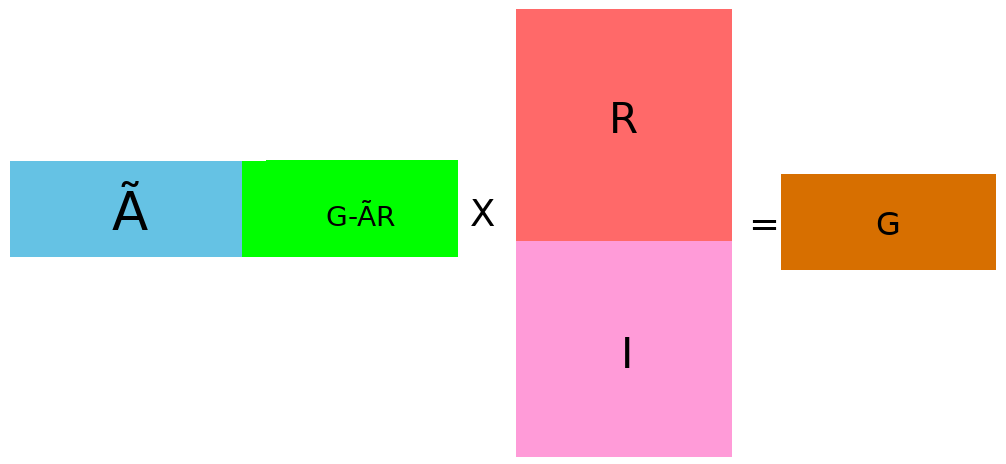
\includegraphics[height=3cm]{imagens/micciancio.png}
    
    Para um dado parâmetro de segurança, a matriz $G$ e seu tamanho são constantes. Portanto, o tamanho de $I$ e $G-\overline{A}R$ também vai ser fixo.
    
    Temos então liberdade para ajustar o número de colunas de $\overline{A}$ conforme for necessário para a segurança do esquema. Mas quanto maior for esse número de colunas, maior deverá ser o número de linhas do trapdoor $R$.
    \end{block}
    
\end{frame}

    \begin{frame}{Função com Trapdoor de Micciancio}

\textbf{Teorema: }Se a função Hash de Ajtai for uma função de mão única, a função com trapdoor de Micciancio que utilizar a mesma matriz como sendo $\overline{A}$ também é uma função de mão única.

    \textbf{Prova (esboço): }Para todo adversário $\mathcal{A}$ que tenta inverter $F$, podemos gerar um novo adversário $\mathcal{B}$ que inverte $H_A$:
    
    \begin{algorithm}[H]
    \SetAlgoLined
    \KwIn{$\lambda=n, \Lambda=Encode(n, m, q, A)$, $t_1 \in \mathbb{Z}_q^n$}
    \KwResult{$\overrightarrow{m_1}$  tal que $A\overrightarrow{m_1} \mod q=t_1$}
    $G \leftarrow \textrm{GerarG}(\lambda, \Lambda)$\;
    $R\leftarrow \textrm{Trapdoor}(\lambda, \Lambda)$\;
    $\mathcal{PK}\leftarrow \textrm{Encode}(\begin{bmatrix}A&G-AR\end{bmatrix})$\;
    $\overrightarrow{m*} \leftarrow^{\$} \mathbb{Z}_q^{w}$\;
    $\overrightarrow{t_2} \leftarrow (G-\overline{A}R)\overrightarrow{m*}$\;
    $\overrightarrow{m} \leftarrow^{\$}\mathcal{A}(\lambda, \Lambda, \overrightarrow{t_1}+\overrightarrow{t_2})$\;
    $\overrightarrow{m_1}||\overrightarrow{m_2} \leftarrow \overrightarrow{m}$ (\textrm{com}\   $\overrightarrow{m_1}\in\mathbb{Z}_q^m)$\;
    \textbf{retorne}\ $\overrightarrow{m_1}$\;
    \caption{Adversário $\mathcal{B}$ que inverte a Hash de Ajtai $H_A$}
\end{algorithm}

\end{frame}

\begin{frame}{Função com Trapdoor de Micciancio}
\textbf{Prova (cont.):} 
\begin{itemize}
\item Se $\mathcal{A}$ retornou uma resposta certa,  então $\begin{bmatrix}A&G-AR\end{bmatrix}(\overrightarrow{m_1}||\overrightarrow{m_2})=\overrightarrow{t_1}+\overrightarrow{t_2}$.
    
\item Como $\overrightarrow{t_2} = (G-AR)\overrightarrow{m*}$, se $\overrightarrow{m_2}=\overrightarrow{m*}$, então: $A\overrightarrow{m_1} + (G-AR)\overrightarrow{m_2} = A\overrightarrow{m_1} + t_2 = t_1+t_2$. Portanto, $A\overrightarrow{m_1} = t_1$ e retornamos com sucesso uma inversa da hash $H_A$.
\item Portanto: $Pr[\mathcal{B}\ \textrm{inverte}\ H_A] \geq Pr[\mathcal{A}\ \textrm{inverte}\ F]\cdot Pr[\overrightarrow{m_2}=\overrightarrow{m*}]$
\item O valor $\overrightarrow{m_2}$ é garantidamente uma solução para o sistema de equações representado por $(G-AR)\overrightarrow{x}=\overrightarrow{c}$. O número de valores que são solução não é superpolinomial. Portanto, $Pr[\overrightarrow{m_2}=\overrightarrow{m*}]$ não é negligível.
\end{itemize}
\end{frame}

\begin{frame}{Função com Trapdoor de Micciancio}
\textbf{Prova (cont.):} Temos então que se conseguirmos um algoritmo eficiente que inverte $F$ com probabilidade não-negligível, então também teríamos um algoritmo eficiente que inverte a hash de Ajtai $H_A$ com chance não-negligível.

Mas pela nossa hipótese, não existiria tal algoritmo. Portanto, não há algoritmo capaz de inverter $F$ se isso for verdade. \qed

\end{frame}

\end{document}